\documentclass[journal]{IEEEtran}
\usepackage{graphicx}
\usepackage[scriptsize]{caption}
\renewcommand{\arraystretch}{1.1}

\begin{document}

\newcommand{\labtitlegen}{
    \twocolumn[{
    \begin{center}
        \LARGE\labtitle \\ \bigskip \large\name \\ \bigskip
        \labsection \\ 
        \textbf{TA} \\ \taname \\% \bigskip \textbf{Lab Partners} \\
%        \partnername
    \end{center}
    }]
}

%% Change these variables
\newcommand{\labtitle}{Experiment 5: Thick and Thin Lenses}
\newcommand{\name}{604-296-523}
\newcommand{\labsection}{Section 2, Wednesday 8AM}
\newcommand{\labdate}{February 18, 2015}
\newcommand{\taname}{Elwin Martin}
\newcommand{\partnername}{Kari Kawashima}


%% This creates your lab cover page.
\labtitlegen

\newcommand{\mval}[3]{$#1 \pm #2 #3$}

\section{Introduction}

The index of refraction of a material can be measured by using Snell's law, $
n_1 sin(\theta _1) = n_2 sin(\theta 2) $, in two distinct ways - by finding the
critical angle and allowing one of the sines to go to one, or by taking the
measurements at an arbitrar angle and calculating the result. We will use both
methods in this lab, and compare their relative advantages.

The properties of thick lenses will also be measured, including the focal
lengths of individual lenses, magnifications of arrays of lenses, and spherical
aberrations. These properties are relevant to the study of thin lenses, since
thin lenses only follow their respective laws approximately.

The focal lengths of several thin lenses will be measured, and used to check
several properties - the effective focal length of an array of thin lenses, and
the formation of images by a thin lens. Both of these properties are
approximately described by the basic thin-lens equations, and may have
systematic errors relating to imperfections in the lenses.

\section{Results}

To measure the index of refraction of the plastic, a single beam of light was
used. We traced the outline of the plastic, and traced the incoming and
outgoing light beams. Figure~\ref{fig:refraction} shows the traced incoming
light beam, as well as the extrapolated path the light took inside the
material. 

\begin{figure}[ht!]
\centering
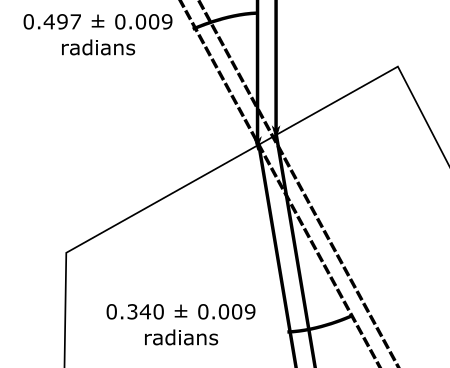
\includegraphics[width=40mm]{refract.png}
\caption{Diagram of refraction, with labeled angles. Reflected light was
omitted, but it reflected relative to the normal with an identical angle of
$0.497 \pm 0.009$ radians.}
\label{fig:refraction}
\end{figure}

Measuring the critical angle was done with an identical setup, by simply
rotating the surface until the exit angle on the opposite side was $\pi / 2$
radians. The critical angle was the incident angle on the inside of the
plastic. The critical angle was measured to be $0.72 \pm 0.03$ radians. The
uncertainty on this angle is higher because near the critical angle, the
effects of the frequency of light on index of refraction become significant -
the beam begins to split into a rainbow, and there is no clear point at which
the entire beam is totally internally reflected. For the purposes of this
measurement, we used the point at which no visible light was re-emitted.

We measured the focal lengths of the thick lenses by first aligning the ray box
such that all emerging light came out strictly parallel. Then, using the baffle
box to get three parallel beams, we allowed the parallel beams to pass through
the thick lenses. Since they entered the lenses parallel to each other, they
emerged converging at the focal point.

\begin{figure}[ht!]
\centering
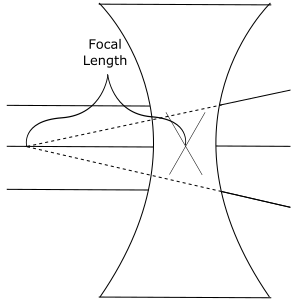
\includegraphics[width=40mm]{focallen.png}
\caption{Setup used to measure focal point of thick lenses. Parallel rays
emitted by ray box, and split into three with baffles.}
\label{fig:focallen}
\end{figure}

Figure~\ref{fig:focallen} shows this measurement for the concave lens. This is
the only diverging lens, so the light rays diverged from the focal point behind
the lens, and it was necessary to extrapolate backwards to find the focal
point. The convex and plano-convex rays both converged in front of the lens.
The distances from all three focal points to the center of their respective
lenses were measured, and are shows in Table 1.

\begin{table}[ht]
    \centering
    \caption*{\normalsize{Thick-Lens Focal Lengths}}
    \scalebox{1.1}{
        \begin{tabular}{|l|l|}
            \hline
            Lens & Focal Length (cm) \\ \hline
            Convex & $6.00 \pm 0.05$ \\ \hline
            Concave & $3.70 \pm 0.05$ \\ \hline
            Plano-Convex & $10.90 \pm 0.05$ \\ \hline
        \end{tabular}
    }
    \medskip
    \caption*{Table 1: Focal lengths of the three thick lenses.}
\end{table}

The same process was used to measure spherical aberration, but with five
parallel rays instead of two. The five rays were passed through the convex
lens. The three inner rays had a focal length of $6.00 \pm 0.05$ cm, as
previously measured, while the outer two rays converged at $5.50 \pm 0.05$ cm.

\begin{figure}[ht!]
\centering
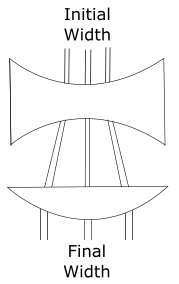
\includegraphics[width=40mm]{magnification.png}
\caption{Setup used to measure magnification of thick lenses in series.}
\label{fig:magnification}
\end{figure}

In addition, we measured the magnification effects of passing the light through
two lenses in conjunction. We first used the concave lens followed by the
plano-convex one, which magnifies the image as shown in
Figure~\ref{fig:magnification}. We then reverse the order to produce
demagnification. All measurements are shown in Table 2.

\begin{table}[ht]
    \centering
    \caption*{\normalsize{Thick-Lens Magnification Measurements}}
    \scalebox{1.1}{
        \begin{tabular}{|l|l|l|}
            \hline
            Type & Initial Width (cm) & Final Width (cm) \\ \hline
            Magnification & $2.0 \pm 0.05$ & $4.15 \pm 0.05$ \\ \hline
            Demagnification & $1.95 \pm 0.05$ & $0.95 \pm 0.05$ \\ \hline
        \end{tabular}
    }
    \medskip
    \caption*{Table 2: Image sizes of concave and plano-convex lenses, first
    in that order, then in reverse order.}
\end{table}

We measured the focal point of thin lenses by shining two parallel laser beams
through them near the center, and finding the distance at which they converged.
This measurement was taken for three separate lenses, here labeled A, B, and C.
The parallel beams were created by shining a laser through a beam splitter -
two semi-reflective surfaces parallel to each other. Properly aligned, both
surfaces reflect the beam, with the offset being the distance between the
surfaces. The measurements are shown in Table 3.

We then used lenses A and C in conjunction, placing them $3.00 \pm 0.05$ cm
from each other, and measured the total focal length of the combination. It
turned out to be TODO. Also, a sphere of diameter 2.54 cm was used as a lens,
and the focal length from the surface of the sphere was measured.

\begin{table}[ht]
    \centering
    \caption*{\normalsize{Thin-Lens Focal Lengths}}
    \scalebox{1.1}{
        \begin{tabular}{|l|l|}
            \hline
            Lens & Focal Length (cm) \\ \hline
            A & $12.9 \pm 0.2$ \\ \hline
            B & $8.7 \pm 0.2$ \\ \hline
            C & $36.0 \pm 0.2$ \\ \hline
            A + C & $21.9 \pm 0.2$ \\ \hline
            Sphere & $0.6 \pm 0.1$ \\ \hline
        \end{tabular}
    }
    \medskip
    \caption*{Table 3: Focal lengths of multiple thing lenses, measured by
    converging two parallel laser beams.}
\end{table}

The uncertainty in focal length for each lens was found by moving the screen
gradually, and seeing the points at which the dots converged, and the point at
which they diverged. That distancewas taken to be twice the uncertainty, and
the central value was taken to be the focal length. 

The last measurement taken was the effects of thin lenses on image formation.
Lens A from the previous measurements was taken, with a focal length of $12.9
\pm 0.2$ cm. It was placed before an object - in this case, a backlit
transparent grating, with a spacing of 1mm. The image was found by moving a
dark blue screen behind the lens until the image came into focus.

Table 4 shows varying distances at which the image was in focus, as well as the
magnification in each case. The magnification was taken by measuring the
distance of 6 grid squares in the image, which would have a spacing of 0.6 cm
in the actual grid. The ratio between this measurement and 0.6 cm is the
magnification of the lens.

\begin{table}[ht!]
    \centering
    \caption*{\normalsize{Thin-Lens Image Distances}}
    \scalebox{1.1}{
        \begin{tabular}{|l|l|l|}
        \hline
        Object (cm)  &  Image (cm)   &  Grid Width (cm)  \\ \hline
        $30.1 \pm 0.1$ & $23   \pm 0.1$ & $0.075 \pm 0.008$ \\ \hline
        $24.6 \pm 0.1$ & $28.6 \pm 0.1$ & $0.133 \pm 0.008$ \\ \hline
        $22   \pm 0.1$ & $33.8 \pm 0.1$ & $0.167 \pm 0.008$ \\ \hline
        $20   \pm 0.1$ & $39.6 \pm 0.1$ & $0.233 \pm 0.008$ \\ \hline
        $18.7 \pm 0.1$ & $46.5 \pm 0.1$ & $0.267 \pm 0.008$ \\ \hline
        $18.4 \pm 0.1$ & $48.3 \pm 0.1$ & $0.300 \pm 0.008$ \\ \hline
        \end{tabular}
    }
    \medskip
    \caption*{Table 4: Magnification of thin lens at varying object/image
    distances.}
\end{table}

\section{Analysis}

The index of refraction can be found using the incident and refracted light
using Snell's law.

\begin{equation}
\label{snells}
n_1 sin(\theta _1) = n_2 sin(\theta 2)
\end{equation}

Using Equation~\ref{snells}, the index of refraction of the material is

\begin{displaymath}
n_2 = n_1 \frac{sin(\theta _1)}{sin(\theta _2)}
\end{displaymath}

The value of $n_1$ is taken to be one, as it is very close to that in air.
Using these assumptions and the values in Figure~\ref{fig:refraction}, the
index of refraction in the material is $1.43 \pm 0.02$.

According to these measurements, the critical angle must then be $0.77 \pm
0.03$ radians. This is in reasonable agreement with the measured value of $0.72
\pm 0.03$ radians - that value was taken when every frequency was completely
internally reflected, which means it will differ slightly from the theoretical
value assuming identical indices of refraction for all frequencies.

The thick lenses measured in Table 2 had a magnification value of $2.1 \pm
0.1$, and a demagnification value of $0.49 \pm 0.03$.

The combination of thin lenses had a focal length different from either of its
component lenses. The new system can be treated as a new lens, with a new focal
length of

\begin{displaymath}
\frac{1}{f} = \frac{1}{f_1} + \frac{1}{f_2} - \frac{d}{f_1 + f_2}
\end{displaymath}

Where $f_1$ and $f_2$ are the focal lengths of the two component lenses, and d
is the separation between the lenses. Using the relation above, and the
measured values for the focal points and separation ($12.9 \pm 0.2$ cm, $36.0
\pm 0.2$ cm, and $3.00 \pm 0.05$ cm), the predicted combined focal length is
$22.8 \pm 0.8$ cm. This matches well with the observed value of $21.9 \pm 0.2$
cm - though the uncertainty ranges nearly don't overlap, the agreement is
within 4\%. There are plenty of factors that could account for the difference -
namely, aberrations in the thin-lens equations.

The image distance found with the thin lens can be verified against the
thin-lens approximation, which takes the form

\begin{displaymath}
\frac{1}{f} = \frac{1}{o} + \frac{1}{i}
\end{displaymath}

Where o is the object distance and i is the image distance. Table 5 shows the
predicted image distances at the given object distances, as well as the
computed magnifications at each object distance. The predicted image distances
also have computed percentages error between them and the real distances in
Table 4.

\begin{table}[ht!]
    \centering
    \caption*{\normalsize{Thin-Lens Image Predictions}}
    \scalebox{1.0}{
        \begin{tabular}{|l|l|l|l|}
        \hline
        Object (cm)  & $Image_{predicted}$ (cm) & \% Error & Magnification \\ \hline
        $30.1 \pm 0.1$ & $22.6 \pm 0.2$ & 1.9  \% & $0.8 \pm 0.1$ \\ \hline
        $24.6 \pm 0.1$ & $27.1 \pm 0.3$ & 5.3  \% & $1.3 \pm 0.1$ \\ \hline
        $22.0 \pm 0.1$ & $31.2 \pm 0.3$ & 8.0  \% & $1.7 \pm 0.2$ \\ \hline
        $20.0 \pm 0.1$ & $36.3 \pm 0.4$ & 8.6  \% & $2.3 \pm 0.2$ \\ \hline
        $18.7 \pm 0.1$ & $41.6 \pm 0.4$ & 11.1 \% & $2.7 \pm 0.3$ \\ \hline
        $18.4 \pm 0.1$ & $43.2 \pm 0.4$ & 11.2 \% & $3.0 \pm 0.3$ \\ \hline
        \end{tabular}

    }
    \medskip
    \caption*{Table 5: Magnifications and predirected image distances of thin
    lens at varying object distances.}
\end{table}

The predicted image distances converge with the measured image distances as the
distance decreases (and as the obejct distance increases). This could
potentially be due to various factors, though it appears to not be due to
measurement error - the bias is always such that the predirected distance is
smaller than the measured distance. The most likely reason is spherical
aberration in the thin lens, causing the effective focal length to change with
decreasing object distance (as was seen in the thick lens). The magnification
rates do match the theory - they increase with decreasing object length, and
switch from magnification to demagnification when the object and image
distances are both equal to twice the focal length.

\section{Conclusion}

The critical angle measurement and prediction different by approximately 7\%,
likely caused by the use of polychromatic light. The index of refraction used
to calculate the theoretical critical angle was calculated when the
contribution of light frequency to index of refraction was minimal, whereas the
real critical angle measurement ended up separating the light into individual
wavelengths. This caused the measured value to be significantly smaller than
the predicted value.

The thick-lens abberation measurement showed that spherical aberrations can
cause the outer part of a lens to have an effectively shorter focal length than
the inner part - in this case, by 8\%.

This could explain the systematic bias observed in image distances formed by a
thin lens. The focal length was measured at exactly the focal length, and using
a particular portion of the lens. If the inner portion was used, the measured
focal length would be smaller than the effective focal length of the entire
lens, causing the corresponding predictions to be smaller than the real values. 

The combination of thin lenses was the most reliable measurement, likely
because the same portions of the lenses were used in measuring the individual
focal lengths and the new effective focal length. This minimized the effects of
spherical aberrations.

\end{document}


